% for notes environment
\usepackage{xsavebox}
\usepackage{hyperref}
\usepackage{graphicx}
\usepackage{luatexja}
\usepackage[hiragino-pro,deluxe,nfssonly,jis2004]{luatexja-preset}
\usepackage{fontspec}
\usepackage{epigraph}
\usepackage{etoolbox}
\usepackage{tikz}
\usepackage{framed}
\usepackage{mathtools}
\usepackage{listings}
\usepackage{libertine}
\usepackage[libertine]{newtxmath}
\usepackage{bxcoloremoji}
\usepackage{xcolor}
\usepackage{diagbox}
\usepackage{caption}
\usepackage{appendixnumberbeamer}
\usepackage{multirow}
\usepackage{xpatch}
\usepackage{multicol}
\usepackage{tabularx}

\usetikzlibrary{fit}

\setmonofont{CMU Typewriter Text}

\definecolor{links}{HTML}{2A1B81}
\hypersetup{colorlinks,linkcolor=,urlcolor=links}

\usetheme{Boadilla}
\usecolortheme{seahorse}
% \usefonttheme{serif}


\xpatchcmd{\itemize}
  {\def\makelabel}
  {\ifnum\@itemdepth=1\relax
     \setlength\itemsep{1.2ex}% separation for first level
   \else
     \ifnum\@itemdepth=2\relax
       \setlength\itemsep{0.8ex}% separation for second level
       \setlength\topsep{1.2ex}
     \else
       \ifnum\@itemdepth=3\relax
         \setlength\itemsep{0.05ex}% separation for third level
         \setlength\topsep{0.8ex}
   \fi\fi\fi\def\makelabel
  }
 {}
 {}

\setbeamercolor{page number in head/foot}{bg=blue!10}
\setbeamertemplate{footline}{%
  \leavevmode%
  \hbox{%
    \begin{beamercolorbox}[wd=.3\paperwidth,ht=2.25ex,dp=1ex,center]{author in head/foot}%
      \usebeamerfont{author in head/foot}\insertshortauthor\hspace*{1ex}(\insertshortinstitute)
    \end{beamercolorbox}%
    \begin{beamercolorbox}[wd=.2\paperwidth,ht=2.25ex,dp=1ex,center]{title in head/foot}%
      \usebeamerfont{title in head/foot}\insertshorttitle
    \end{beamercolorbox}%
    \begin{beamercolorbox}[wd=.4\paperwidth,ht=2.25ex,dp=1ex,center]{date in head/foot}%
      \insertshortdate{} @ \InsertConference
    \end{beamercolorbox}%
    \begin{beamercolorbox}[wd=.1\paperwidth,ht=2.25ex,dp=1ex,center]{page number in head/foot}%
      \insertframenumber{} / \inserttotalframenumber\hspace*{1ex}
    \end{beamercolorbox}}%
  \vskip0pt%
}

\beamertemplatenavigationsymbolsempty

\setbeamertemplate{bibliography item}{\insertbiblabel}
\setbeamersize{description width=1cm}
\setbeamertemplate{items}[circle]
\setbeamertemplate{section in toc}[circle]
\setbeamertemplate{subsection in toc}{%
  \leavevmode\leftskip=2em
  {%
    \usebeamerfont*{itemize item}%
    \usebeamercolor{subsection number projected}%
    \color{bg}%
    \raise1.25pt\hbox{\donotcoloroutermaths$\bullet$}}%
  \hskip1.5ex\inserttocsubsection\par}

% Definitions for the title page
\newcommand*{\GitHub}[1]{%
  \gdef\InsertGitHub{#1}%
}
\newcommand*{\Email}[1]{%
  \gdef\InsertEmail{\href{mailto:#1}{#1}}%
}
\newcommand*{\Conference}[1]{%
  \gdef\InsertConference{#1}%
}
\setbeamerfont{title}{size=\huge, series=\bfseries, family=\mcfamily\rmfamily}
\setbeamercolor{title}{bg=white}
\setbeamerfont{subtitle}{size=\Large, series=\mdseries, family=\gtfamily\sffamily}
\setbeamerfont{email}{size=\scriptsize, family=\ttfamily}
\setbeamercolor{email}{bg=white}
\setbeamerfont{date}{shape=\itshape, family=\rmfamily}
\setbeamerfont{vc}{size=\scriptsize, family=\ttfamily}
\setbeamercolor{vc}{bg=white}

\renewcommand{\figurename}{Fig}

\input{vc.tex}

\setbeamertemplate{title page}
{%
  \vbox{}
  \vfill
  \begingroup
    \centering
    \hrulefill\par%
    \vskip1ex\par%
    \begin{beamercolorbox}[sep=0pt,center,shadow=false,rounded=true]{title}
      \vfill
      \usebeamerfont{title}\inserttitle\par%
      \ifx\insertsubtitle\@empty%
      \else%
        \vskip0.5ex%
        {\usebeamerfont{subtitle}\usebeamercolor[fg]{subtitle}\insertsubtitle\par}%
      \fi%
      \vfill  
    \end{beamercolorbox}%
    \hrulefill\par%
    \vskip2ex%
    \begin{beamercolorbox}[sep=0pt,center,shadow=false,rounded=true]{author}
      \usebeamerfont{author}\insertauthor
    \end{beamercolorbox}
    \begin{beamercolorbox}[sep=0pt,center,shadow=false,rounded=true]{email}
      \usebeamerfont{email}\InsertEmail
    \end{beamercolorbox}
    \vskip0.1ex
    \begin{beamercolorbox}[sep=5pt,center,shadow=false,rounded=true]{institute}
      \usebeamerfont{institute}\insertinstitute
    \end{beamercolorbox}
    \begin{beamercolorbox}[sep=5pt,center,shadow=false,rounded=true]{date}
      \usebeamerfont{date}\insertdate \normalfont @ \InsertConference
    \end{beamercolorbox}
    \begin{beamercolorbox}[sep=0pt,center,shadow=false,rounded=true]{vc}
      \usebeamerfont{vc}
      \url{https://github.com/\InsertGitHub} (\texttt{\GITAbrHash})
    \end{beamercolorbox}
    % {\centering
    %   \href{https://creativecommons.org/licenses/by-nc/4.0/}{%
    %     \includegraphics[width=0.1\textwidth]{img/by-nc.pdf}%
    %   }%
    % }
    {\usebeamercolor[fg]{titlegraphic}\inserttitlegraphic\par}
  \endgroup
  \vfill
}
\setbeamertemplate{blocks}[rounded][shadow=false]

% ============ ここを消すとNote消える ================
% \mode<handout>{%
%   \usepackage{pgfpages}
%   \setbeameroption{show notes on second screen=right}
%   \setbeamertemplate{note page}{%
%     \vspace{2ex}\insertnote%
%   }
% }
% ============ ここを消すとNote消える ================


\renewcommand{\kanjifamilydefault}{\gtdefault}

\setbeamertemplate{caption}[numbered]
\resetcounteronoverlays{lstlisting}
\definecolor{bluegray}{rgb}{0.4, 0.6, 0.8}
\DeclareCaptionFormat{listing}{{\color{bluegray}\lstlistingname}#2#3}
\captionsetup[lstlisting]{format=listing, font={footnotesize}}
\captionsetup[figure]{name={図}}
\captionsetup[table]{name={表}}
\setbeamerfont{footnote}{size=\scriptsize}

\setmonofont[Ligatures=TeX]{CMU Typewriter Text}

\setbeamertemplate{items}[circle]

\newfontfamily\quotefont[Ligatures=TeX]{Linux Libertine O} % selects Libertine as the quote font

\newcommand*\quotesize{60} % if quote size changes, need a way to make shifts relative
% Make commands for the quotes
\newcommand*{\openquote}
   {\tikz[remember picture,overlay,xshift=0em,yshift=-3ex]
   \node (OQ) {\quotefont\fontsize{\quotesize}{\quotesize}\selectfont``};\kern0pt}

\newcommand*{\closequote}[1]
  {\tikz[remember picture,overlay,xshift=1ex,yshift={#1}]
   \node (CQ) {\quotefont\fontsize{\quotesize}{\quotesize}\selectfont''};}

\newcommand*\shadedauthorformat{\emph} % define format for the author argument

% Now a command to allow left, right and centre alignment of the author
\newcommand*\authoralign[1]{%
  \if#1l
    \def\authorfill{}\def\quotefill{\hfill}
  \else
    \if#1r
      \def\authorfill{\hfill}\def\quotefill{}
    \else
      \if#1c
        \gdef\authorfill{\hfill}\def\quotefill{\hfill}
      \else\typeout{Invalid option}
      \fi
    \fi
  \fi}
% wrap everything in its own environment which takes one argument (author) and one optional argument
% specifying the alignment [l, r or c]
%
\newenvironment{shadequote}[2][l]%
{\hspace{0.5ex}
\authoralign{#1}
\ifblank{#2}
   {\def\shadequoteauthor{}\def\yshift{-1ex}\def\quotefill{\hfill}}
   {\def\shadequoteauthor{\par\authorfill\shadedauthorformat{#2}}\def\yshift{3ex}}
\begin{quote}\normalfont\openquote}
{\shadequoteauthor\quotefill\closequote{\yshift}\end{quote}}

\makeatletter
\def\@fnsymbol#1{\ensuremath{\ifcase#1\or \dagger\or \ddagger\or
   \mathsection\or \mathparagraph\or \|\or **\or \dagger\dagger
   \or \ddagger\ddagger \else\@ctrerr\fi}}
\makeatother

\renewcommand{\thefootnote}{\fnsymbol{footnote}}
\renewcommand{\thempfootnote}{\fnsymbol{mpfootnote}}
\newcommand\ballcircle[1]{%
  {%
    \usebeamercolor{enumerate item}%
    \tikzset{beameritem/.style={circle,inner sep=0,minimum size=2ex,text=enumerate item.bg,fill=enumerate item.fg}}%
    \tikz[baseline=(n.base)]\node(n)[beameritem]{\sffamily#1};%
  }%
}
\newcommand\ballref[1]{%
  \ballcircle{\ref{#1}}%
}

\usetikzlibrary{calc}
\usetikzlibrary{shapes.callouts} 

\pgfkeys{%
    /calloutquote/.cd,
    width/.code                   = {\def\calloutquotewidth{#1}},
    position/.code                = {\def\calloutquotepos{#1}}, 
    author/.code                  = {\def\calloutquoteauthor{#1}},
    at/.code                      = {\def\calloutquoteat{#1}},
    sign/.code                    = {\def\calloutquotesign{#1}},
    /calloutquote/.unknown/.code  = {\let\searchname=\pgfkeyscurrentname
                                      \pgfkeysalso{\searchname/.try=#1,                        
                                      /tikz/\searchname/.retry=#1},\pgfkeysalso{\searchname/.try=#1,
                                      /pgf/\searchname/.retry=#1}
                                    }
}

\makeatletter

\newsavebox\temp@simple@callout@author@box
\newcommand\calloutquote[2][]{%
  \pgfkeys{/calloutquote/.cd,
    width    = 5cm,
    position = {(0.5,-0.2)},
    at       = {(0,0)},
    author   = {},
    sign     = {+}
  }%
  \pgfqkeys{/calloutquote}{#1}%
  \sbox{\temp@simple@callout@author@box}{\mbox{%
    \begin{tabular}{l}
      \calloutquoteauthor%
    \end{tabular}
  }}%
  \node[thin, draw=black!50, rectangle callout,callout relative pointer={\calloutquotepos},align=center,text width=\calloutquotewidth,/calloutquote/.cd,
     #1] (tmpcall) at \calloutquoteat {#2};
  \node at ($ (tmpcall.pointer) - (-\calloutquotesign0.5\wd\temp@simple@callout@author@box,0.7\ht\temp@simple@callout@author@box) $) {\calloutquoteauthor};
}

\newsavebox\temp@simple@callout@box
\newcommand{\simplecallout}[4][{}]{%
  \sbox{\temp@simple@callout@box}{\mbox{%
    \begin{tabular}{l}
      #4%
    \end{tabular}
  }}%
  \begin{center}%
    \begin{tikzpicture}%
      \calloutquote[width=1.05\wd\temp@simple@callout@box,position={(#2.5,-0.2)},fill=#3,rounded corners,author={#1},sign=#2]{
        #4%
      }%
    \end{tikzpicture}%
  \end{center}
}

\makeatother
\newfontfamily{\listingfont}[Scale=0.85]{Menlo}
\definecolor{dkgreen}{rgb}{0,0.6,0}
\definecolor{gray}{rgb}{0.5,0.5,0.5}
\definecolor{mauve}{rgb}{0.58,0,0.82}

\makeatletter
\lst@CCPutMacro\lst@ProcessOther {"2D}{\lst@ttfamily{-{}}{-{}}}
\@empty\z@\@empty
\makeatother

\lstdefinestyle{csharp}{
  numbers=left,
  language=[Sharp]C
}

\lstdefinestyle{cil}{
  numbers=left,
  language=CIL
}

\lstdefinestyle{plain}{
  basicstyle=\listingfont\scriptsize,
  language=Plain,
  showstringspaces=false,
  showtabs=false,
  stringstyle=\listingfont\scriptsize\color{mauve},
  tabsize=2
}

\lstdefinestyle{sh}{
  numbers=left,
  language=sh
}

\lstdefinestyle{c}{
  numbers=left,
  language=C
}

\lstdefinestyle{python}{
  numbers=left,
  language=Python
}

\lstdefinestyle{asm-x86}{
  numbers=left
}

\lstdefinestyle{pseudo-code}{
  numbers=left,
  keywords=[6]{for,from,to,endfor,while,endwhile}
}

\lstdefinestyle{bitcoin-script}{
  mathescape=true
}

\lstset{
  basicstyle=\listingfont,
  frame=single,
  xleftmargin=2em,
  xrightmargin=1em,
  breaklines=true
}

\lstdefinestyle{scala}{
  basicstyle=\listingfont\scriptsize,
  breakatwhitespace=false,
  language=scala,
  captionpos=b,
  commentstyle=\listingfont\scriptsize\color{dkgreen},
  extendedchars=true,
  xleftmargin=1em,
  xrightmargin=1em,
  keepspaces=true,
  keywordstyle=\listingfont\scriptsize\color{blue},
  emphstyle=\listingfont\scriptsize\color{cyan},
  rulecolor=\listingfont\scriptsize\color{black},
  showspaces=false,
  showstringspaces=false,
  showtabs=false,
  stringstyle=\listingfont\scriptsize\color{mauve},
  tabsize=2
}

\lstdefinestyle{go}{
  basicstyle=\listingfont\scriptsize,
  breakatwhitespace=false,
  language=go,
  captionpos=b,
  commentstyle=\listingfont\scriptsize\color{dkgreen},
  extendedchars=true,
  xleftmargin=1em,
  xrightmargin=1em,
  keepspaces=true,
  keywordstyle=\listingfont\scriptsize\color{blue},
  emphstyle=\listingfont\scriptsize\color{cyan},
  rulecolor=\listingfont\scriptsize\color{black},
  showspaces=false,
  showstringspaces=false,
  showtabs=false,
  stringstyle=\listingfont\scriptsize\color{mauve},
  tabsize=2
}

\lstdefinestyle{js}{
  basicstyle=\listingfont\scriptsize,
  breakatwhitespace=false,
  language=JavaScript,
  captionpos=b,
  commentstyle=\listingfont\scriptsize\color{dkgreen},
  extendedchars=true,
  xleftmargin=1em,
  xrightmargin=1em,
  keepspaces=true,
  keywordstyle=\listingfont\scriptsize\color{blue},
  emphstyle=\listingfont\scriptsize\color{cyan},
  rulecolor=\listingfont\scriptsize\color{black},
  showspaces=false,
  showstringspaces=false,
  showtabs=false,
  stringstyle=\listingfont\scriptsize\color{mauve},
  tabsize=2
}

\lstdefinestyle{css}{
  basicstyle=\listingfont\scriptsize,
  breakatwhitespace=false,
  language=CSS,
  captionpos=b,
  commentstyle=\listingfont\scriptsize\color{dkgreen},
  extendedchars=true,
  xleftmargin=1em,
  xrightmargin=1em,
  keepspaces=true,
  keywordstyle=\listingfont\scriptsize\color{blue},
  emphstyle=\listingfont\scriptsize\color{cyan},
  rulecolor=\listingfont\scriptsize\color{black},
  showspaces=false,
  showstringspaces=false,
  showtabs=false,
  stringstyle=\listingfont\scriptsize\color{mauve},
  tabsize=2
}

\lstdefinestyle{html}{
  basicstyle=\listingfont\scriptsize,
  breakatwhitespace=false,
  language=HTML5,
  captionpos=b,
  commentstyle=\listingfont\scriptsize\color{dkgreen},
  extendedchars=true,
  xleftmargin=1em,
  xrightmargin=1em,
  keepspaces=true,
  keywordstyle=\listingfont\scriptsize\color{blue},
  emphstyle=\listingfont\scriptsize\color{cyan},
  rulecolor=\listingfont\scriptsize\color{black},
  showspaces=false,
  showstringspaces=false,
  showtabs=false,
  stringstyle=\listingfont\scriptsize\color{mauve},
  tabsize=2
}

\lstdefinelanguage{Plain}{
  morestring=[b]",
  morestring=[b]'
}

\lstdefinelanguage{scala}{
  morekeywords={abstract,case,catch,class,def,%
    do,else,extends,false,final,finally,%
    for,if,implicit,import,match,mixin,%
    new,null,object,override,package,%
    private,protected,requires,return,sealed,%
    super,this,throw,trait,true,try,%
    type,val,var,while,with,yield},
  moreemph={Byte,Short,Int,Long,Float,Double,Char,
    String,Boolean,Unit,Null,Nothing,Any,AnyRef,
    Left,Right,Either},
  otherkeywords={=>,<-,<\%,<:,>:,\#,@},
  sensitive=true,
  morecomment=[l]{//},
  morecomment=[n]{/*}{*/},
  morestring=[b]",
  morestring=[b]',
  morestring=[b]"""
}

\lstdefinelanguage{golang}%
  {morekeywords=[1]{package,import,func,type,struct,return,defer,panic,%
     recover,select,var,const,iota},%
   morekeywords=[2]{string,uint,uint8,uint16,uint32,uint64,int,int8,int16,%
     int32,int64,bool,float32,float64,complex64,complex128,byte,rune,uintptr,%
     error,interface},%
   morekeywords=[3]{map,slice,make,new,nil,len,cap,copy,close,true,false,%
     delete,append,real,imag,complex,chan,},%
   morekeywords=[4]{for,break,continue,range,go,goto,switch,case,fallthrough,if,%
     else,default,},%
   morekeywords=[5]{Println,Printf,Error,Print,},%
   sensitive=true,%
   morecomment=[l]{//},%
   morecomment=[s]{/*}{*/},%
   morestring=[b]',%
   morestring=[b]",%
   morestring=[s]{`}{`},%
}

\lstdefinelanguage{JavaScript}{%
  keywords={typeof, new, true, false, catch, function, return, null, catch, switch, var, if, in, while, do, else, case, break},
  keywordstyle=\color{blue}\bfseries,
  ndkeywords={class, export, boolean, throw, implements, import, this},
  ndkeywordstyle=\color{darkgray}\bfseries,
  identifierstyle=\color{black},
  sensitive=false,
  comment=[l]{//},
  morecomment=[s]{/*}{*/},
  commentstyle=\color{purple}\ttfamily,
  stringstyle=\color{red}\ttfamily,
  morestring=[b]',
  morestring=[b]"
}

\lstdefinelanguage{CSS}{
  keywords={url},
  morekeywords={@import},
  keywordstyle=\color{blue},
  morecomment=[s]{/*}{*/}
}

\lstdefinelanguage{HTML5}{
    sensitive=true,
    keywords={%
    % JavaScript
    typeof, new, true, false, catch, function, return, null, catch, switch, var, if, in, while, do, else, case, break,
    % HTML
    html, title, meta, style, head, body, script, canvas,
    % CSS
    border:, transform:, -moz-transform:, transition-duration:, transition-property:,
    transition-timing-function:
    },
    % http://texblog.org/tag/otherkeywords/
    otherkeywords={<, >, \/},   
    ndkeywords={class, export, boolean, throw, implements, import, this},   
    comment=[l]{//},
    % morecomment=[s][keywordstyle]{<}{>},  
    morecomment=[s]{/*}{*/},
    morecomment=[s]{<!}{>},
    morestring=[b]',
    morestring=[b]",    
    alsoletter={-},
    alsodigit={:}
}
\newenvironment{notes}
  {%
    \begin{xlrbox}{NotesBox}
    \begin{minipage}{.95\textwidth}
    \small\rmfamily\mcfamily
    \begin{itemize}
    \setlength{\itemindent}{0em}
    \setlength{\footnotesep}{5mm}
  }{%
    \end{itemize}
    \end{minipage}
    \end{xlrbox}
    \note{\theNotesBox}}

\def\AtSOne#1\csod{%
	\begin{array}{c|}
		\hline
		#1\\
		\hline
	\end{array}
}%
\def\AtSTwo#1,#2\csod{%
	\begin{array}{c|c|}
		\hline
		#1 & #2\\
		\hline
	\end{array}
}%
\def\AtSThree#1,#2,#3\csod{%
	\begin{array}{c|c|c|}
		\hline
		#1 & #2 & #3\\
		\hline
	\end{array}
}%
\def\AtSFour#1,#2,#3,#4\csod{%
	\begin{array}{c|c|c|c|}
		\hline
		#1 & #2 & #3 & #4\\
		\hline
	\end{array}
}%
\def\AtSFive#1,#2,#3,#4,#5\csod{%
	\begin{array}{c|c|c|c|c|}
		\hline
		#1 & #2 & #3 & #4 & #5\\
		\hline
	\end{array}
}%
\def\AtSSix#1,#2,#3,#4,#5,#6\csod{%
	\begin{array}{c|c|c|c|c|c|}
		\hline
		#1 & #2 & #3 & #4 & #5 & #6\\
		\hline
	\end{array}
}
\newcommand{\SOne}[1]{\AtSOne#1\csod}
\newcommand{\STwo}[1]{\AtSTwo#1\csod}
\newcommand{\SThree}[1]{\AtSThree#1\csod}
\newcommand{\SFour}[1]{\AtSFour#1\csod}
\newcommand{\SFive}[1]{\AtSFive#1\csod}
\newcommand{\SSix}[1]{\AtSSix#1\csod}
\newcommand\card[1]{\boxed{#1}}
\newcommand\heartcard{\card{\color{red}{♥}}}
\newcommand\clubcard{\card{♣}}
\newcommand\commitedcard{\card{\,?\,}}
% \def\yescards{\heartcard\,\heartcard\,\clubcard}
% \def\nocards{\heartcard\,\clubcard\,\clubcard}
% \def\threecommitedcards{\commitedcard\,\commitedcard\,\commitedcard}
% \def\threeheartcards{\heartcard\,\heartcard\,\heartcard}
% \def\threeclubcards{\clubcard\,\clubcard\,\clubcard}

\newcommand\ce[1]{%
  \coloremojiucs{#1}
}

\newcommand*{\lstitem}[1]{
  \setbox0\hbox{\lstinline{#1}}
  \item[\usebox0]
}

\presetkeys{todonotes}{inline, noinlinepar}{}

\title[奢り・割勘プロトコル]{%
  奢り・割勘プロトコル
}
\subtitle{}
\author[吉村 優]{%
  吉村 優(\textsc{Yoshimura} Hikaru)
}
\Email{hikaru\_yoshimura@r.recruit.co.jp}
\date[January 25, 2023]{%
  \oldstylenums{January 25, 2023}
}
\Conference{社会人語学プロ開2023年3月期4Q部会}
\institute[\InsertEmail]{株式会社リクルート(Recruit Co., Ltd)}
\GitHub{y-yu/fair-or-all-slide}

\begin{document}

\frame{\maketitle}

\section{はじめに}

\begin{frame}
  \frametitle{目次}

  \tableofcontents
\end{frame}

\begin{frame}
  \frametitle{自己紹介}
  
  \begin{columns}
    \begin{column}{0.3\textwidth}
      \begin{center}
        \begin{figure}
          
\includegraphics[width=0.95\textwidth]{img/bird2x.png}
        \end{figure}
      \end{center}
 
      \begin{table}[h]
        \begin{tabular}{ll}
          Twitter & \href{https://twitter.com/\_yyu\_}{@\_yyu\_} \\
          Qiita &  \href{https://qiita.com/yyu}{yyu} \\
          GitHub &  \href{https://github.com/y-yu}{y-yu} \\
        \end{tabular}
      \end{table}
    \end{column}
    \begin{column}{0.7\textwidth}
      \begin{itemize}
        \item 筑波大学 情報学群 情報科学類卒(2011-15,学士)
        \begin{itemize}
          \item プログラム論理研究室、WORD編集部
        \end{itemize}
        
        \item ドワンゴ ニコニコ動画 アカウントチーム

        \item 未踏ターゲット2018(ゲート式量子コンピュータ)

        \item CTF(\url{https://urandom.team/})
        \begin{itemize}
          \item SECCON CTF 2022で世界57位(国内20位)
        \end{itemize}

        \item プログラミング
        \begin{itemize}
          \item Scala, \LaTeX, Rust, Go, Swift
        \end{itemize}
      \end{itemize}
    \end{column}
  \end{columns}
\end{frame}

\section{奢り・割勘問題}

\begin{frame}
  \frametitle{奢り・割勘問題}

  \begin{figure}[h]
    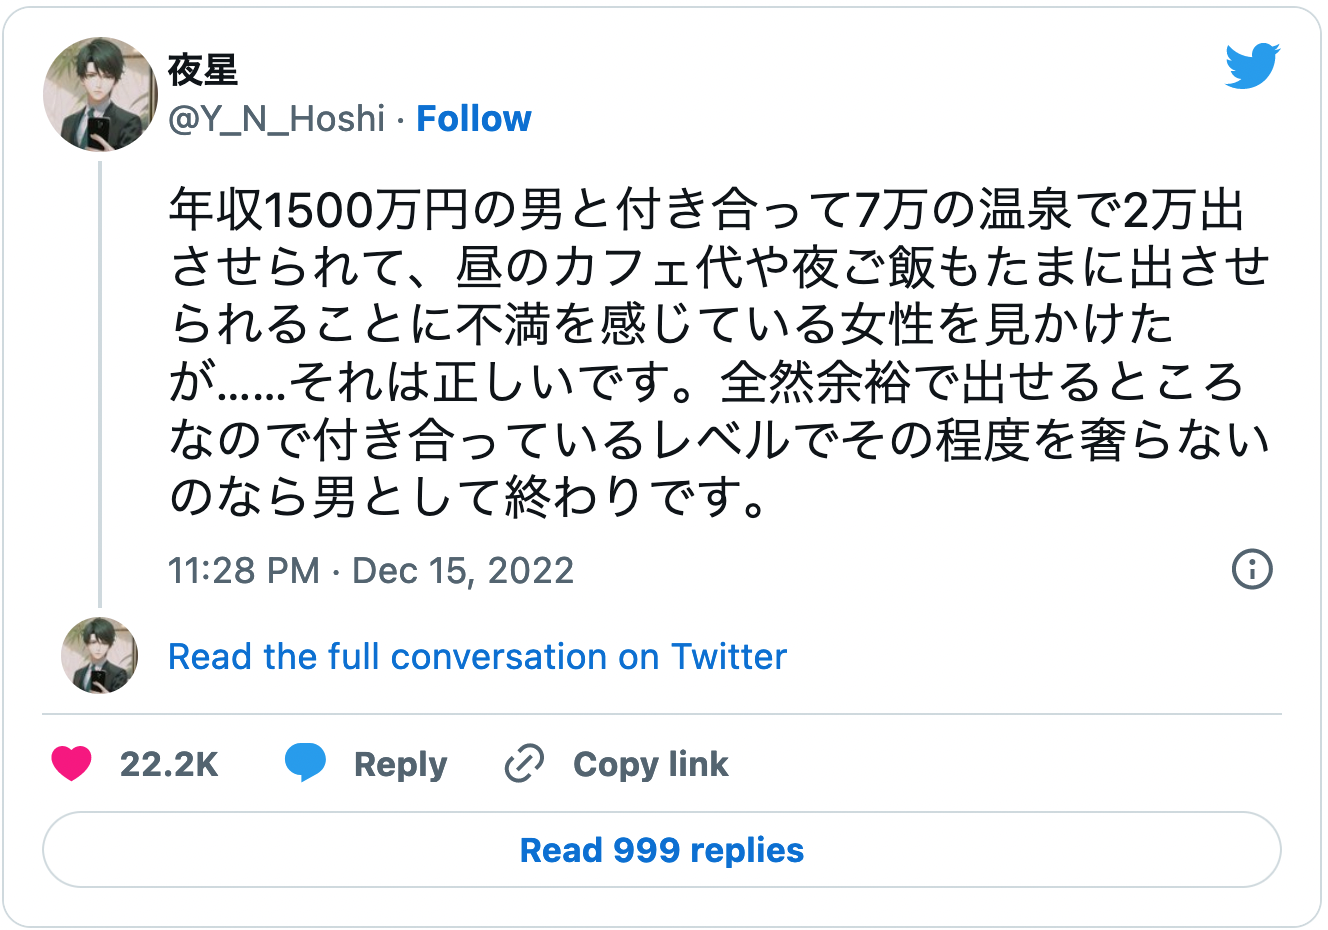
\includegraphics[width=0.65\textwidth]{./img/twitter.png}\cite{Y_N_Hoshi}
  \end{figure}
\end{frame}

\begin{frame}
  \frametitle{奢り・割勘問題}

  \begin{shadequote}[r]{}
    \begin{center}
      アリスとボブの飲食費について下記のいずれにするか決定する問題
      \begin{enumerate}
        \item ボブが全額を奢る
        \item 割勘とする
      \end{enumerate}
    \end{center}
  \end{shadequote}

  \begin{columns}
    \begin{column}{0.5\textwidth}
      \centering
      \emph{アリス(Alice)}

      \begin{figure}[h]
        
\includegraphics[height=0.4\textheight]{img/alice.png}
      \end{figure}
    \end{column}
   
    \begin{column}{0.5\textwidth}
      \centering
      \emph{ボブ(Bob)}

      \begin{figure}[h]
        
\includegraphics[height=0.4\textheight]{img/bob.png}
      \end{figure}
    \end{column}
  \end{columns}
\end{frame}

\section{従来手法}

\newcommand{\facesize}{1cm}

\begin{frame}
  \frametitle{従来手法 \ballcircle{1}コイントス}

  \begin{enumerate}
    \item アリス・ボブの間でコイントスを行う

    \item その結果に応じて次のように決定する
    \begin{description}
      \item[結果が表] ボブが全額奢る
      \item[結果が裏] 割勘
    \end{description}
  \end{enumerate}

  \pause
  \simplecallout[%
    {
\includegraphics[width=\facesize]{./img/bob_face.png}}%
  ]{+}{orange!10}{%
    当事者たちの意見が何も反映されないためプライバシーは完全\ce{:person_gesturing_ok:}
  }

  \simplecallout[%
    {
\includegraphics[width=\facesize]{./img/alice_face.png}}%
  ]{-}{cyan!10}{%
    しかしゲーム性は全くない
  }
\end{frame}

\begin{frame}
  \frametitle{従来手法 \ballcircle{1}コイントス}

  \begin{columns}
    \begin{column}{0.6\textwidth}
      \simplecallout[%
        {
\includegraphics[width=\facesize]{./img/alice_face.png}}%
      ]{+}{cyan!10}{%
        そもそもこのゲームはアリスが有利\ce{:smiling_imp:}
      }

      \simplecallout[%
       {
\includegraphics[width=\facesize]{./img/bob_face.png}}%
      ]{-}{orange!10}{%
        そもそも不公平なゲームなので、\\
        50:50ではおもしろくない
      }
    \end{column}
    \begin{column}{0.4\textwidth}
      \begin{itemize}
        \item ボブが支払うのは50\% or 100\%だが
        \item 一方でアリスは0\% or 50\%
      \end{itemize}
    \end{column}
  \end{columns}
\end{frame}

\newcolumntype{Y}{>{\centering\arraybackslash}X}
\begin{frame}
  \frametitle{従来手法 \ballcircle{2}公平な第三者によるAND計算}

  \pause
  \begin{enumerate}
    \item アリスとボブは公平な第三者チャーリーに$\text{\textbf{希望}} \in \{\text{奢り}, \text{割勘}\}$を渡す
    \item チャーリーはアリス・ボブの希望を次の表\ref{tbl:and_table}に基づいてAND演算する
    \item チャーリーが結果を2人に通知する
  \end{enumerate}

  \begin{table}[h]
    \caption{奢り・割勘AND演算}
    \label{tbl:and_table}
    \begin{tabularx}{0.7\textwidth}{@{}| Y | Y || Y |@{}}
      \hline
      アリス & ボブ & 結果 \\ \hline
      割勘  & 割勘 & 割勘 \\ \hline
      割勘  & 奢り & 割勘 \\ \hline
      奢り  & 割勘 & 割勘 \\ \hline
      奢り  & 奢り & 奢り \\ \hline
    \end{tabularx}
  \end{table}

  \begin{itemize}
    \item ボブは$\frac{3}{4}$の確率で50\%の支払い、
    $\frac{1}{4}$の確率で100\%の支払いなので期待値は$\frac{5}{8}$(62.5\%)の支払い

    \item 同様の計算でアリスは期待値$\frac{3}{8}$(37.5\%)の支払い
  \end{itemize}
\end{frame}

\begin{frame}
  \frametitle{従来手法 \ballcircle{2}公平な第三者を用いたAND計算}
  
  \begin{columns}
    \begin{column}{0.6\textwidth}
      \simplecallout[%
        {
\includegraphics[width=\facesize]{./img/bob_face.png}}%
      ]{+}{orange!10}{%
        そもそもチャーリーが信頼できるのか?
      }

      \simplecallout[%
        {
\includegraphics[width=\facesize]{./img/alice_face.png}}%
      ]{-}{cyan!10}{%
        \noindent
        次のケース\ce{:point_down:}で\textbf{情報リーク}が生じる!\\
        \hbox to 0.5\textwidth{%
          \vbox{%
            \begin{enumerate}
              \item アリスが奢り、ボブは割勘を希望
              \item アリスが割勘、ボブは奢りを希望\label{enum:bob_detect}
              \item アリスが奢り、ボブは奢りを希望
            \end{enumerate}
          }
        }
      }
    \end{column}
    \begin{column}{0.4\textwidth}
      \begin{itemize}
        \item AND計算なので片方の入力と結果から、残った入力が逆算できる場合がある
      \end{itemize}
    \end{column}
  \end{columns}
\end{frame}

\begin{frame}
  \frametitle{従来手法 \ballcircle{2}公平な第三者によるAND計算}

  \begin{columns}
    \begin{column}{0.6\textwidth}
      \simplecallout[%
        {
\includegraphics[width=\facesize]{./img/bob_face.png}}%
      ]{+}{orange!10}{%
        希望が場合によっては流出するのは\\
        ゲーム性とみなすことができそう\ce{:thinkig_face:}
      }

      \simplecallout[%
        {
\includegraphics[width=\facesize]{./img/alice_face.png}}%
      ]{-}{cyan!10}{%
        しかし\ballcircle{2}の方法では\\
        \textbf{高目の支払いを強いられた側}の\\
        情報がリークすることがある\ce{:rage:}
      }
    \end{column}
    \begin{column}{0.4\textwidth}
      \begin{itemize}
        \item たとえば「アリスが割勘・ボブは奢りを希望」のとき、
        結果は割勘となる。
        ボブは奢りを回避してさらにアリスの上品さも知ることができる

        \item しかしアリスはボブの希望を知ることはできない
      \end{itemize}
    \end{column}
  \end{columns}
\end{frame}

\section{提案手法}

\begin{frame}
  \frametitle{コイントスとAND計算のハイブリッドプロトコル}

  \begin{columns}
    \begin{column}{0.6\textwidth}
      \simplecallout[%
        {
\includegraphics[width=\facesize]{./img/bob_face.png}}%
      ]{+}{orange!10}{%
        表\ref{tbl:choice_and_info_leak}のようにランダムを導入したうえで、\\
        不本意な結果を強いられた側だけが\\
        相手の希望を得るというのはどうか?
      }

      \simplecallout[%
        {
\includegraphics[width=\facesize]{./img/alice_face.png}}%
      ]{-}{cyan!10}{%
        互いの希望がマッチした場合には\\
        情報が一切リークしない
      }
    \end{column}
    \begin{column}{0.4\textwidth}
      \begin{table}[h]
        \caption{奢り・割勘と情報リーク}
        \label{tbl:choice_and_info_leak}
        \begin{tabular}{|l|l|c|c|}
          \hline
          アリス & ボブ & 結果   & 情報 \\ \hline
          割勘  & 割勘 & 割勘   & \dagger \\ \hline
          割勘  & 奢り & ランダム & \ddagger \\ \hline
          奢り  & 割勘 & ランダム & \ddagger  \\ \hline
          奢り  & 奢り & 奢り   & \dagger \\ \hline
        \end{tabular}

        \footnotetext[1]{お互いの希望はいずれもリークしない} 
        \footnotetext[2]{結果が奢りの場合はアリスの希望がボブへ、結果が割勘の場合はボブの希望がアリスへリークする}
      \end{table}
    \end{column}
  \end{columns}
\end{frame}

\begin{frame}
  \frametitle{コイントスとAND計算のハイブリッドプロトコル}

  \simplecallout[%
    {
\includegraphics[width=\facesize]{./img/bob_face.png}}%
  ]{+}{orange!10}{%
    期待値的にはボブが不公平なままだが、\\
    もし不本意に奢った場合はアリスのがめつさが分かる
  }

  \simplecallout[%
    {
\includegraphics[width=\facesize]{./img/alice_face.png}}%
  ]{-}{cyan!10}{%
    このときアリスはボブの奢りが本意か不本意か分からないが、奢られを得る
  }
\end{frame}

\begin{frame}
  \frametitle{コイントスとAND計算のハイブリッドプロトコル}

  \simplecallout[%
    {
\includegraphics[width=\facesize]{./img/alice_face.png}}%
  ]{+}{cyan!10}{%
    逆にアリスが不本意に割勘となってしまった場合、\\
    ボブの希望は割勘だと特定する
  }

  \simplecallout[%
    {
\includegraphics[width=\facesize]{./img/bob_face.png}}%
  ]{-}{orange!10}{%
    しかしこのときボブはアリスの希望が分からない
  }
\end{frame}

\begin{frame}
  \frametitle{手順}

  このプロトコルはチャーリー(\emph{trusted third party})\textbf{なし}で達成できる

  \pause
  \begin{columns}
    \begin{column}{0.6\textwidth}
      \begin{enumerate}
        \item アリス・ボブに2枚のカード\heartcard,\clubcard を配る\footnote{%
          これらのカードはトランプのようにいずれも裏が\commitedcard となっており、
          裏向きになった状態でどちらのカードなのか特定することができない
        }
        \item アリス・ボブは表\ref{tbl:card_meaning}に従って
        希望を裏向き\commitedcard にして提出する\label{enum:cards_commited}

        \item \ballref{enum:cards_commited}で提出されたカードをシャッフルする
        
        \item どちらか1枚をドローして表向きにする。カードを表\ref{tbl:card_meaning}させた
        ものがプロトコルの結果となる
      \end{enumerate}
    \end{column}
    \begin{column}{0.4\textwidth}
      \begin{table}[h]
        \renewcommand{\arraystretch}{1.5}
        \caption{カードの意味}
        \label{tbl:card_meaning}
        \begin{tabularx}{0.9\textwidth}{@{}| Y | Y |@{}}
          \hline
          カード & 意味 \\ \hline
          \heartcard & ボブの奢り \\ \hline
          \clubcard & 割勘 \\ \hline
        \end{tabularx}
      \end{table}
    \end{column}
  \end{columns}
\end{frame}

\begin{frame}
  \frametitle{ケーススタディ}

\end{frame}

\section{まとめ}

\begin{frame}
  \frametitle{まとめ}

  \pause
  \begin{itemize}
    \item<+-> 簡単なプロトコルで奢り・割勘問題に決着をつけられるかもしれない

    \item<+-> 今回紹介した技術は``Covert Lottery\cite{covert_lottery}''という名前が付いている

    \item<+-> 今回は2人だったが、これを多人数拡張すると別のゲームに使えるかもしれない
  \end{itemize}
\end{frame}

\section*{参考文献}
\begin{frame}%[allowframebreaks]
  \frametitle{参考文献}
  \nocite{*}
  \bibliographystyle{junsrt_url}
  \bibliography{ref}
\end{frame}

\begin{frame}
  \centering
  {\Huge Thank you for the attention!}
\end{frame}

\end{document}
